\documentclass[12pt]{article}
\usepackage[english]{babel}
\usepackage[letterpaper,top=2cm,bottom=2cm,left=3cm,right=3cm,marginparwidth=1.75cm]{geometry}
\usepackage{amsmath}
\usepackage{graphicx}
\usepackage{hyperref}
\title{STAT-UB 103 Homework 9}
\author{Ishan Pranav}
\date{April 30, 2023}
\renewcommand{\thesubsection}{\thesection.\alph{subsection}}
\renewcommand{\theenumi}{\alph{enumi}}
\begin{document}
\maketitle
\section{A study}
\begin{enumerate}
\item Without looking at the data, we can expect a negative relationship between a person's intelligence test score and the age at which they spoke their first word.
\item Yes, as expected, the plot in \autoref{fig:scoreagescatterplot} indicates a negative relationship between age and score.
\begin{figure}[h]
\begin{center}
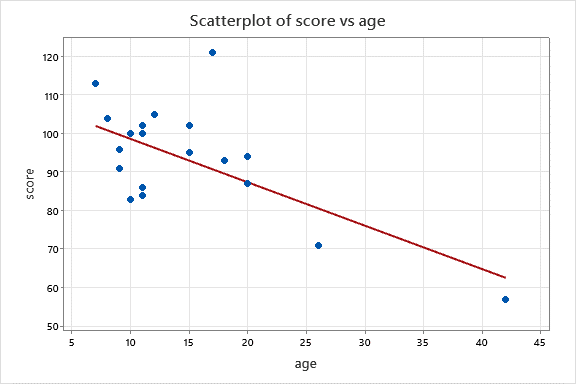
\includegraphics[width=3.5in]{src/images/score-age-scatterplot.png}
\end{center}
\caption{Scatterplot for intelligence test score (response) and age at which first words were spoken (predictor).\label{fig:scoreagescatterplot}}
\end{figure}
\item See \autoref{fig:scoreageregression}.
\begin{figure}[!h]
\begin{center}
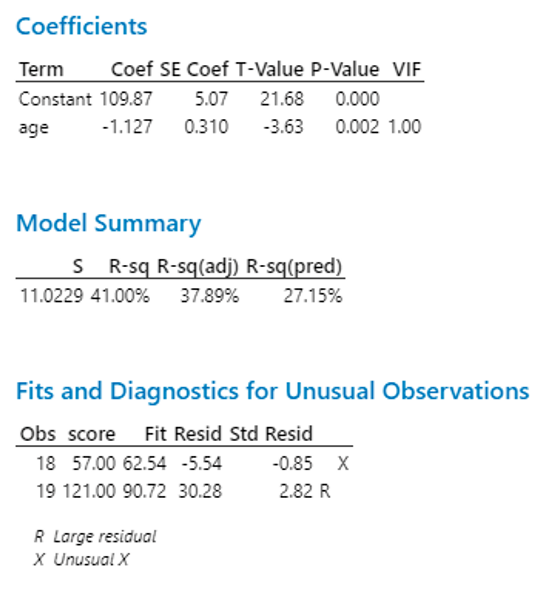
\includegraphics[width=3in]{src/images/score-age-regression.png}
\end{center}
\caption{Linear regression analysis for intelligence test score (response) and age at which first words were spoken (predictor).\label{fig:scoreageregression}}
\end{figure}
\item
\[H_0:\beta_1=0.\]
\[H_1:\beta_1\neq 0.\]
\[P(t=-3.63\,|\,H_0)\approx0.002.\]
There is evidence at the one-half-percent significance level that score is related to age.
\item
\[H_0:\beta_1=0.\]
\[H_1:\beta_1<0.\]
\[P(t=-3.63\,|\,H_0)\approx\frac{0.002}{2}\approx 0.001.\]
Given that the null hypothesis is true, the probability of obtaining a Student $t$-statistic as extreme as (or more extreme than) $-3.63$ is approximately 0.1 percent. Since 0.001 is smaller than the significance level ($\alpha=0.005$), there is sufficient evidence to reject the null hypothesis at the half-percent significance level. There is evidence that score is related to age.
\item \[r^2\approx 0.4100\]

Approximately 41 percent of the variation in a person's intelligence test score can be explained by variations in the age at which they spoke their first words using a least-squares regression line. This suggests that the linear relationship is moderate.
\item The point (42, 57) is a leverage point because its leverage is 0.65161, which is greater than $\frac{2(k+1)}{n}$. The Cook's distance for this point is 0.678112, which is less than 1, meaning that it is not necessarily a bad leverage point. However, it is still significantly higher than the others: The next-highest is 0.081498. Visually, the point is a good leverage point, but it is still worth evaluating the point.
\item 
\[H_0:\beta_1=0.\]
\[H_1:\beta_1\neq 0.\]
\[P(t=-1.51\,|\,H_0)\approx 0.149.\]

After removing the point, the $P$-value is no longer statistically significant, meaning that without the point (42, 57), we cannot conclude beyond a reasonable doubt that there is a linear relationship between age and score.

\[r^2\approx 0.1122.\]

After removing the point, the $r^2$ coefficient of determination has decreased by almost 30 percentage points. This means that the point (42, 57) was extremely influential on the least-squares regression model.
\item Yes, it may be justifiable to remove the point (42, 57) because of its high leverage and influence on the model. Without the point, the linear relationship between age and score is inconclusive.
\end{enumerate}
\end{document}